\documentclass{article}
\usepackage[utf8]{inputenc}
\usepackage{graphicx}
\graphicspath{ {images/} }

\title{MIMD-UI: Testing Guide}

\author{
  Ferreira, Alfredo\\
  \texttt{alfredo.ferreira@tecnico.ulisboa.pt}
  \and
  Calisto, Francisco Maria\\
  \texttt{francisco.calisto@tecnico.ulisboa.pt}
}

\date{May 2017}

\begin{document}

\maketitle

\section{Introduction}

This document aims to describe the protocol of the set of tests that will be performed in the scope of the master's thesis and research papers of the Medical Imaging Multimodality of Breast Cancer Diagnosis User Interface (MIMBCD-UI) project comparing interactive touch environments with traditional environments (mouse and keyboard). The objective of the tests is to compare manipulation techniques in two distinct environments, to understand the techniques and environments that allow a more precise manipulation. With the session, the sessions will be recorded via video on the computer and using a record, heat-map and triggered event tools. It is guaranteed the confidentiality of the recordings, which will be used only for academic purposes.

Each test session is divided into two parts. In one test the traditional environment supported by the interaction with mouse and keyboard and the other a touch environment using touch tablets.

\section{Material}

The material used in the test sessions for both systems consists of:

\begin{itemize}
  \item MacBook Pro: it will allow the user to interact with the keyboard and a wireless mouse;
  \item Wireless Mouse: it will allow the user to interact with a mouse and will complement the keyboard;
  \item Microsoft Surface: to us as a touch environment, it will allow the clinics to interact with a touch user interface;
\end{itemize}

\section{Traditional Technical Description}

To produce this traditional environment, and since we can simulate with a laptop, the mouse and keyboard interaction, we are using a Microsoft Mobile Mouse 4000 together the MacBook Pro (Retina, 13-inch, Early 2015) with a standard integrated key board on the laptop.

\section{Touch Technical Description}

This section aims to summarize a touch technical description of the testing guide where the interaction between a surface user interface in a touch environment will be compared to a traditional one. The user has to handle the tablet more comfortably to interact with the user interface. After that, it accesses the server via a web browser through the tablet, where the user tests are initialized. This model of Microsoft Surface tablet with Windows RT 8.1 allows a comfortable use and a reliable test, since it is an equipment that is updated and in an average range of equipment in terms of what is expected. The specifications are, processor nVidia TEGRA 3 Quad Core 1.30 GHz, 2 GB of RAM and 1250x550 screen resolution.

\section{Traditional Environment}

Traditional interaction remains the most common way to interact with user interfaces on a clinical environment. Unfortunately most of this interaction is made by low profile equipment that make users produce more errors and take more time interacting with those user interfaces.

\section{Touch Environment}

Touch interaction with computationally enhanced surfaces
has received considerable recent attention. Approaches
to the implementation of touch interaction  have allowed for the low cost development of such surfaces, less human errors and better times. This is leading to a number of technology and application innovations.

\clearpage

\section{Interactive Buttons}

The systems have several buttons that allow you to interact or access the same functionality, the Freehand ROI Notification. The buttons are:

\begin{itemize}
  \item Disable
  \item Enable
  \item Active
  \item Deactivate
  \item Back
  \item Clear drawing
  \item Next
\end{itemize}

\section{Procedures}

Each test will take place according to the following structure:

\subsection{Initial Questionnaire}

Prior to the start of the session, participants will be asked to complete a short questionnaire, with the aim of defining their user profile and experience with stereoscopy and other stives. You will be asked to answer the following questions:

\begin{itemize}
  \item Sex, Age, Literacy.
  \item Experience with multi-touch devices (smartphones, tablets, etc).
  \item Experience with Picture Archiving and Communication System (PACS) and if so, which ones.
  \item Experience with Computer-aided Diagnosis (CAD) software and if so, which ones.
\end{itemize}

\clearpage

\subsection{Introduction}

A presentation of the systems and their use and capabilities will be made. They will be presented interactions and will be explained how to interact with the both prototypes, explaining the limitations with regard to hand monitoring.

\subsection{Training Session}

The user will be shown how to annotate and interact in all degrees of freedom. With the aim of enabling users to get their work done before the test tasks. This one training period will be 5 minutes.

\subsection{Execution of Tasks}

Throughout the test session, the user will perform freehand ROI annotation tasks in two environments, the traditional environment and the touch environment. The session will thus be divided into two steps, during which the user will perform 7 tasks in both environments:

1) Access the prototype and go trough the 3 DICOM images.

2) "Activate" the annotations.

3) Start annotate with the freehand function until close the pointing circles. At the end, press "Next" and do the same to image 2 and image 3.

5) "Deactive" the functionality and try to draw again. It will not draw anything since the functionality is deactive.

6) Press "Desable" and see what happens. The lines disappear.

7) Make the lines appear again by pressing "Enable". But this time we won't say this to the user and see if the user understands the mechanic of the interaction.

The order of systems and techniques will be random, however the order of tasks will be pre-established, with incremental difficulty, in which in the first task the user only needs to press any button, in the second task it is necessary to press inside the image, whereas in the last task you must annotate and press next image. In each task, the test objects will be in an initial random state and will be restarted by terminating the application if a previous task has been performed-mind. The task ends when the user understands that he/she has performed the proposed task, or when this is prolonged for a time beyond reasonable.

\clearpage

\subsection{Final Survey}

After completion of the tasks, users will be asked to complete a questionnaire to classify each prototype and technique according to various parameters such as ease of interaction, annotation, fun, etc.

\section{Tasks}

For the accomplishment of the tasks the objects visible in Figure 1 are used. These were chosen, so that there is only one possible way of being annotated, with only the yellow freehand draw annotation.

\begin{figure}[h]
\caption{Example of a Freehand ROI Annotation}
\centering
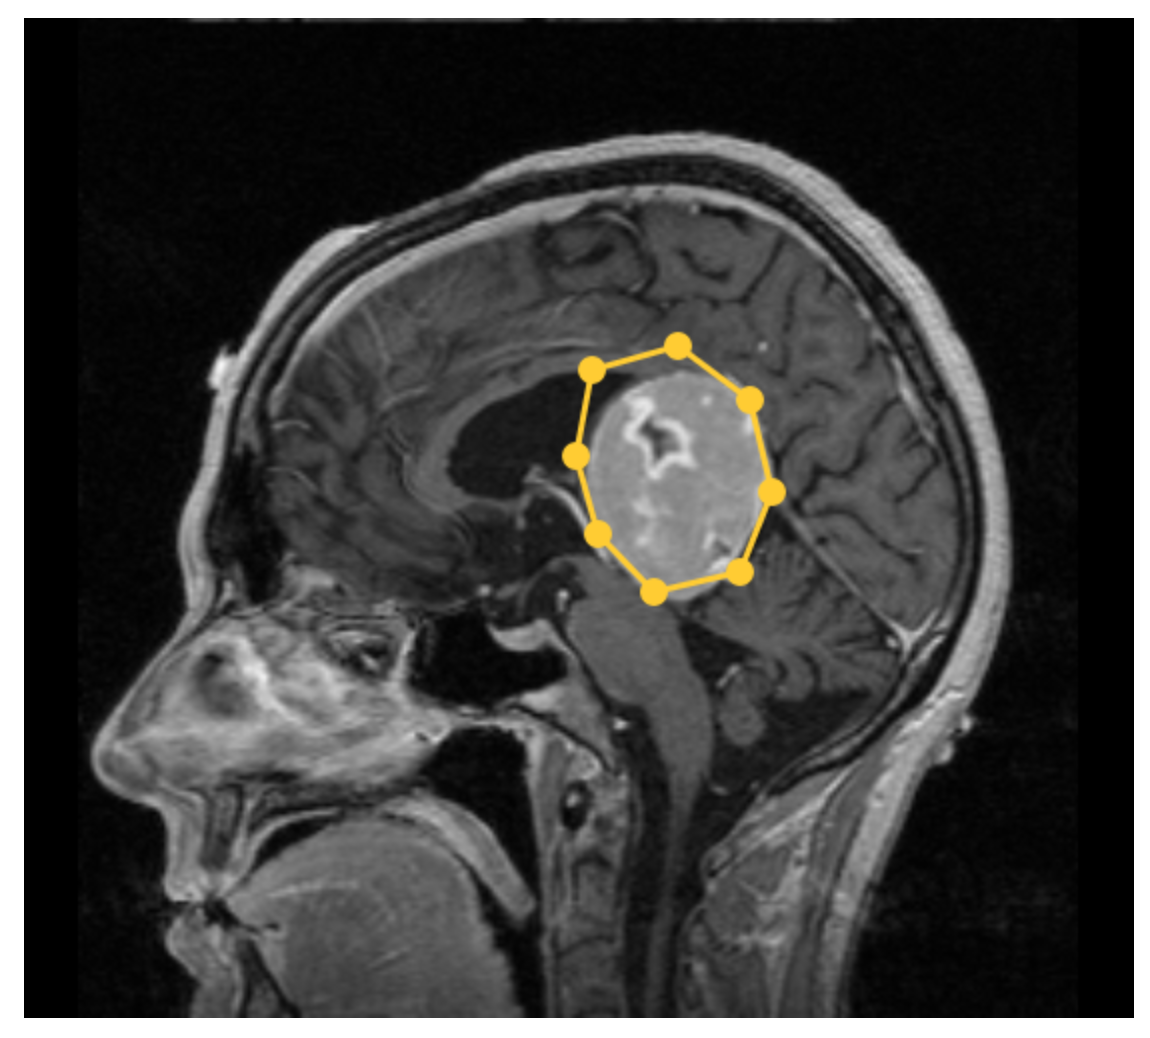
\includegraphics[width=\textwidth]{img1.png}
\end{figure}

\clearpage

The tasks in each environment will be executed in incremental difficulty order.

\begin{figure}[h]
\caption{User Interface Options}
\centering
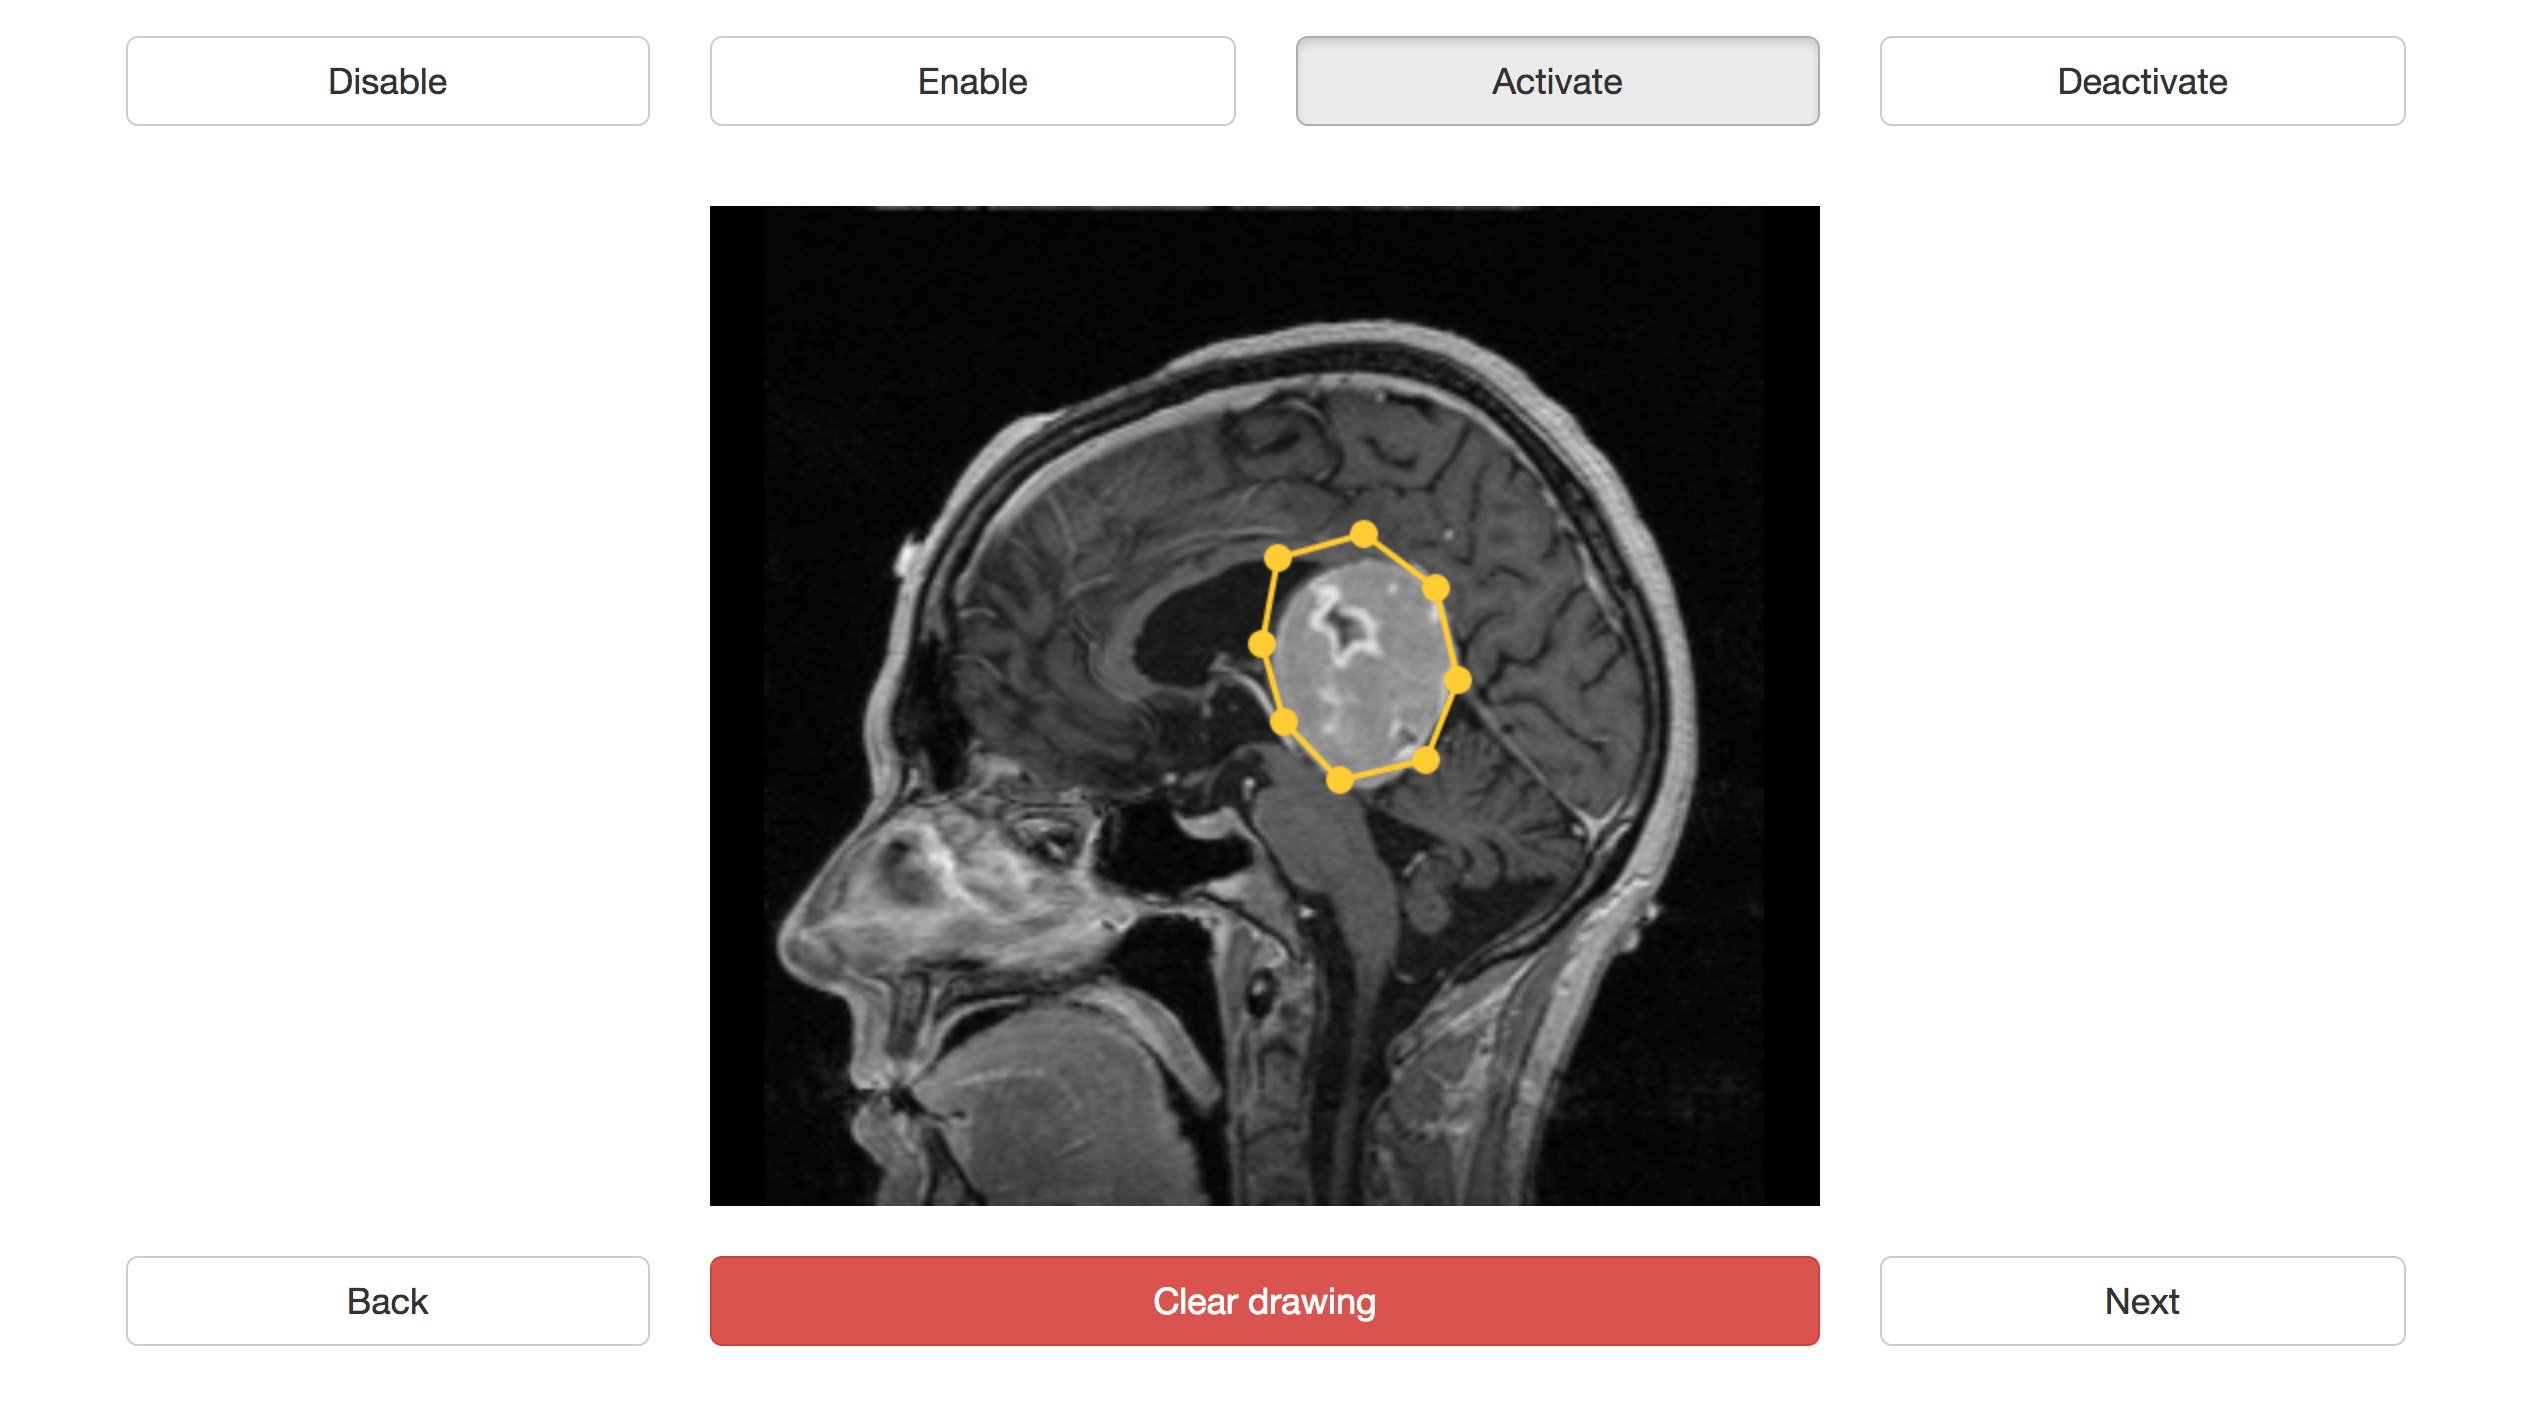
\includegraphics[width=\textwidth]{img2.png}
\end{figure}

In the first task the user only needs to observe and do some basic interaction, in the second task it is necessary to activate the notations and on the third task to draw it. While in the last tasks we won't give the user information about how to do it.

\section{Measurements}

The tests are intended to achieve the following measures:

\begin{itemize}
  \item Number of clicks;
  \item Number of errors;
  \item Number of pressed "Clear drawing" button;
  \item Efficiency;
  \item Time measurement;
  \item Difficulty;
\end{itemize}

\clearpage

Through the questionnaire after the test session, we intend to obtain the answers to the following questions for each environment (for each response a scale of 1 to 5 is given):

\begin{itemize}
  \item Difficulty of interaction in each environment.
  \item Difficulty translating in each environment.
  \item Difficulty performing a freehand ROI in each technique.
  \item Degree of interaction fun in each environment.
  \item Order of preference of each environment.
  \item Degree of tiredness.
  \item Degree of discomfort and disorientation.
\end{itemize}

\end{document}
